% Preamble
\documentclass[a4paper, 12pt]{article}
\usepackage[margin=1in]{geometry} % Set margin
\usepackage{pdfpages} % Insert pdf pages
\usepackage{amssymb,amsmath,amsthm, amsfonts} % Math libraries

% Custom commands
\newcommand{\sub}[1]{\subsection{\underline{#1}}}
\newcommand{\subsub}[1]{\subsubsection{\underline{#1}}}
\newcommand{\?}{\stackrel{?}{=}}
\newcommand{\R}{\ensuremath{\mathbb{R}}}
\newcommand{\F}{\ensuremath{\mathbb{F}}}
\newcommand{\Onef}{\ensuremath{1_{\F}}}
\newcommand{\Zerof}{\ensuremath{0_{\F}}}
\newcommand{\eqbcuz}[1]{\text{~$\stackrel{(#1)}{=}$~}}
\renewcommand{\qed}{$$\blacksquare$$}
\renewcommand{\b}[1]{\textbf{#1}}
\renewcommand{\because}[1]{~\b{(#1)}\\}
\renewcommand{\d}{\ensuremath{\Downarrow\\~}}
\newtheorem{lemma}{Lemma}

% Begin Document %
\begin{document}

% Title Page
\begin{titlepage}
    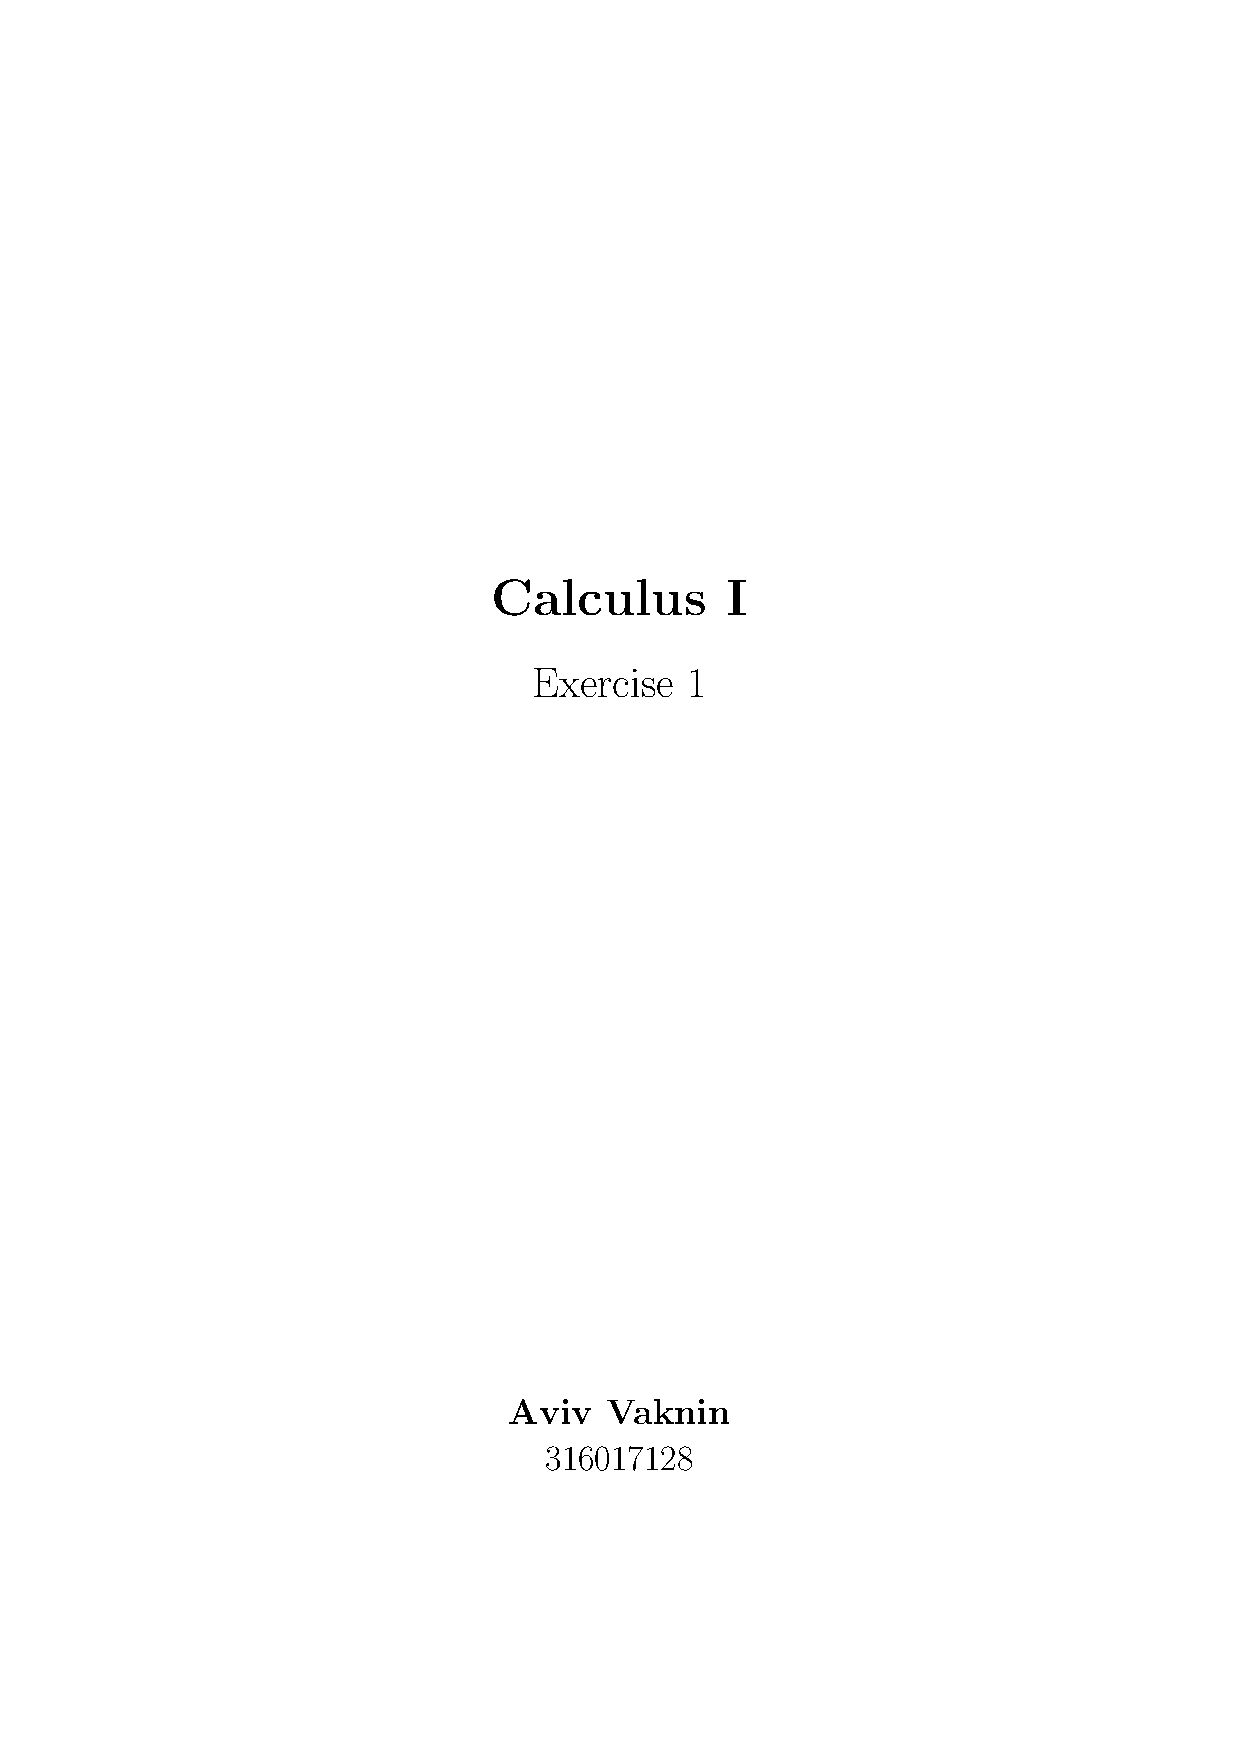
\includepdf{title.pdf}
\end{titlepage}

\section{}
\sub{}
While $i$ and $ii$ are statements, $iii$ isn't a statement,\\
because we haven't received any information about $x$'s value.
\sub{}
    \textit{i})\\
        Statement: $$ \forall{n}\in{\F} ~~ \exists{m}\in{\F} ~\big{|}~ n=m+m $$
        Negated Statement: $$ \exists{n}\in{\F} ~~ \forall{m}\in{\F} ~\big{|}~ n\neq m+m $$
    \textit{ii})\\
        Statement: $$ \forall{m,n}\in{\F} ~~ n=m+m \rightarrow -n=-m-m $$
        Negated Statement: $$ \exists{m,n}\in{\F} ~~ n=m+m ~\land~ -n\neq-m-m $$
\sub{}
    \textit{i})\\
        Statement: $$ \forall{n}\in{\F} ~~ \exists{m}\in{\F} ~\big{|}~ n=m+m $$
        Negated Statement: $$ \exists{n}\in{\F} ~~ \forall{m}\in{\F} ~\big{|}~ n\neq m+m $$

\section{}
\textit{i} is the formal representation of a field's additive inverse axiom, i.e. A4.\\
On the other hand, \textit{ii} states that in the field \F, there's a certain number, $x$,
that if we'll add it to \b{any} other number in \F, we'll receive $0_{\F}$.\\
The two statements are \b{not} logically equal.
\pagebreak

\section{}
\sub{Prove $\forall~a,b \in{\F}~ -(a-b)=(b-a)$}
First, let's find $(a-b)$'s inverse: $$ (a-b)+x=0 $$
We'll add $(b-a)$ to both sides of the equation: $$ (a-b)+(b-a)+x=(b-a) $$
And find the inverse: $$ x = (b-a) $$
Now, we can easily see that $(a-b)$ and $(b-a)$ are the inverses of each other.\\
And due to the additive inverse axiom (A4) : $$ -(a-b) = x = (b-a) $$
\qed

\sub{Prove the 'uniquness of multiplicitive inverse' property}
It is given that $ab, ac=1_{\F}$, and we need to prove that $b=c=a^{-1}$.
\subsub{$ab=1_{\F}$}
According to the multiplicitive inverse property (M4), we can deduct:
$$ b=a^{-1} $$
\subsub{$ac=1_{\F}$}
Exactly as above (M4), we can deduct:
$$ c=a^{-1} $$
Therefore, we can conclude: $$ b=c=a^{-1} $$
\qed
\pagebreak

% 4
\section{$H$ is a set that satisfies all of the field axioms,\\
$H \neq \text{\O}$, $1_H=0_H$\\
Prove that $H$ contains only a single member.}
Adding two $0_H$ should result in a $0_H$, due to axiom A3: $$ 0_H + 0_H = 0_H $$
However, because $1_H=0_H$, it also means that: $$ 1_H + 1_H = 0_H $$
Because of that, we can conculde that no other members exist in $H$, except $1_H=0_H$
\qed

% 5
\section{\F~is an ordered field, prove the following:}

%5.1
\sub{$\forall{x,y} \in{\F}~ 0_{\F}<x<y \iff 0_{\F}<y^{-1}<x^{-1} $}
\subsub{$0_{\F}<x<y ~\Longrightarrow~ 0_{\F}<y^{-1}<x^{-1} $:}
It is given that: $$ x<y $$
We'll multiple both sides of the inequality by 1, using axiom \textit{M4}: $$ xyy^{-1}<yxx^{-1} $$
It is given that $x,y > 0$ therefore we can divide the equation by $xy$: $$ y^-1 < x^-1 $$
\subsub{$0_{\F}<x<y ~\Longleftarrow~ 0_{\F}<y^{-1}<x^{-1} $:}
It is given that: $$ y^{-1}<x^{-1} $$
We'll multiple both sides of the inequality by 1, using axiom \textit{M4}: $$ y^{-1}xx^{-1}<x^{-1}yy^{-1} $$
It is given that $x^-1,y^-1 > 0$ therefore we can divide the equation by $x^-1y^-1$: $$ x<y $$
\qed\pagebreak

%5.2
\sub{$ x,y,z,w \in \F \big{|}~ x<y,~z\leq{w} ~\Longrightarrow~ x+z<y+w$}
It is given that: $$ x<y $$
We'll add $(z+w)$ to both sides, according to axiom \textit{O3}: $$ x+(z+w) < y+(z+w) $$
According to axiom \textit{A1}, we'll rearrange the inequality: $$ (x+z)+w < (y+w)+z $$
It is given that $z \leq w$, therefore if we'll remove $w$ from the left side,
and $z$ from the right side, the inequality should remain correct:
$$ x+z < y+w $$
\qed\pagebreak

%5.3
\sub{$ \forall{x,y} \in{\F}~ (0_{\F}<xy) \iff ((x<0_{\F} \land y<0_{\F}) \lor (0_{\F} < x \land 0_{\F}<y))  $}
\subsub{$ 0_{\F}<xy \Longrightarrow ((x<0_{\F} \land y<0_{\F}) \lor (0_{\F} < x \land 0_{\F}<y))$:}
Due to the ordered field's trichotomy axiom, $x,y$ must be $>0$ or $<0$, 
it is known that $xy>0$ and therefore $x,y \neq 0$ (as proven before).\\
If $x>0$: $$ xy > 0 $$
Let's divide by x: $$ y > 0 $$
Else, if $x<0$: $$ xy > 0 $$
If we divide by x, the $>$ will change to a $<$, as proven previously in exercise 2.5: $$ y < 0 $$
Therefore, we can see that if $xy>0$, $x,y>0$ or $x,y<0$ must be true.

\subsub{$ 0_{\F}<xy \Longleftarrow ((x<0_{\F} \land y<0_{\F}) \lor (0_{\F} < x \land 0_{\F}<y))$:}
First, let's assume that $0_{\F} < x \land 0_{\F}<y$: $$x > 0 $$
According to ordered field's axiom 4, we can multiply both sides of the inequality by $y$: $$ xy > 0 $$
Now, let's assume that $0_{\F} > x \land 0_{\F}>y $: $$x < 0 $$
If we multiply both sides of the equation by y(which is negative), the inequality will change signs: $$ xy > 0 $$
\qed\pagebreak

\sub{Prove:}
$$ 0<b\in{\F}~~\forall{a}\in{\F}~~a^2<b^2 \Longrightarrow -b<a<b $$
Due to the ordered field's trichotomy axiom, $a$ is one of the following:
\begin{itemize}
    \item $a<0$
    \item $a=0$
    \item $a>0$
\end{itemize}
Therefore, we'll need to show that the statement is true for all three.

\subsub{$a=0$:}
$$ b>0 $$
Using the ordered field's $O3$ axiom, we'll subtract $b$ from both sides: $$ b-b > -b $$
Using $A3$: $$ -b < 0 $$
Now, according to transitivity: $$ -b < 0 = a < b $$

\subsub{$a>0$:}
First, we'll need a lemma to help us demonstrate an idea.
\begin{lemma}
    ~\\We want to show that $$ a,b>0 ~~ a^2 > b^2 \Longrightarrow~ a>b $$
    We'll prove that by contraposition: $$ a\leq{b} \Longrightarrow~ a^2\leq{b^2} $$
    We'll multiply the left side by $b$, and by $a$:
    $$ a\leq{b} $$
    $$ a^2\leq{a\cdot{b}} $$
    $$ a\cdot{b}\leq{b^2} $$
    Therefore, according to the transitivity axiom: $$ a^2 \leq{b^2} $$
\end{lemma}
\pagebreak
~\\As shown in the lemma, we know that $b>a$.\\
In addition, it was proven in class that if $b>0$, $-b<0$.\\
Therefore, according to transitivity:
$$ -b < 0 < a < b $$

\subsub{$a<0$:}
I tried to prove that $a>-b$, but failed miserably.
I could really use a hint.

\section{Prove or disprove the following, for $a,b,x,y \in{\F}$:}
\sub{$ab<a+b$}
Let $a,b=0_{\F}$: $$ 0_{\F}\cdot{0_{\F}} < 0_{\F} + 0_{\F} $$
According to Axioms $A3$ and $M3$ it yields the \b{false} statement: $$ 0_{\F} < 0_{\F} $$

\sub{$ x^2<y^2 \Longrightarrow x<y $}
In order to disprove this statement, we need to find $x,y \in{\F}$ such that: $$ x^2<y^2 ~\land~ x \geq y $$
As an example, we can take: $$ x = \Onef$$ $$y=-(\Onef+\Onef) $$
We can see that $x\geq y$.\\
$x^2$: $$ x^2 = \Onef\cdot\Onef=\Onef $$
$y^2$: $$ y^2 = -(\Onef+\Onef)\cdot(-(\Onef+\Onef))=\Onef+\Onef+\Onef+\Onef $$
We can see that $y^2>x^2$, thus, the statement is \b{false}.
\pagebreak

\sub{$ x<y \Longrightarrow x^2<y^2 $}
In order to disprove this statement, we need to find $x,y \in{\F}$ such that: $$ x<y ~\land~ x^2\geq y^2 $$
We can use the same examples from $6.2$, only swapping the $x$ and the $y$: $$ y = \Onef$$ $$x=-(\Onef+\Onef) $$
We can see that $y\geq x$.\\
$y^2$: $$ y^2 = \Onef\cdot\Onef=\Onef $$
$x^2$: $$ x^2 = -(\Onef+\Onef)\cdot(-(\Onef+\Onef))=\Onef+\Onef+\Onef+\Onef $$
We can see that $x^2>y^2$, thus, the statement is \b{false}.

\section{Prove $\forall{a}\in\F~|-a|=|a|$:}
According to the definition of absolute value, there are two different scenarios for $a$:
\subsub{$a \geq 0$:}
Since $a\geq 0$, using the abs definition we'll get: $$ |a| = a $$
According to the ordered field axioms $-a < 0$, and therefore: $$|(-a)| = -(-a) = a$$
We can see that: $$a \geq 0 \Longrightarrow |-a|=|a|=a$$

\subsub{$ a<0 $:}
Since $a<0$, using the abs definition will yield: $$|a| = -a $$
We've previously proved that the negative of a negative is positive, i.e. $-a>0$, therefore:
$$ |-a| = -a $$
We can see that: $$a < 0 \Longrightarrow |-a|=|a|=-a$$
\qed\pagebreak

\section{Prove the following for $a,b\in\F$:}
\sub{$\max(a,b)=\frac{1}{2}(a+b+|a-b|)$}
This splits into three different cases:
\begin{itemize}
    \item $a<b$
    \item $a=b$
    \item $a>b$
\end{itemize}
\subsub{$a<b$:}
$$\max(a,b)=\frac{1}{2}(a+b+|a-b|)$$
Since $a<b$, the term $|a-b|$ is equal to $b-a$, therefore:
$$ \max(a,b)=\frac{1}{2}(a+b+|a-b|) = \frac{1}{2}(a+b+b-a) = \frac{1}{2}(2b) = b $$

\subsub{$a=b$:}
$$\max(a,b)=\frac{1}{2}(a+b+|a-b|)$$
Since $a=b$, the term $|a-b|$ is equal to $0$, therefore:
$$ \max(a,b)=\frac{1}{2}(a+b+0) = \frac{1}{2}(a+b) = \frac{a+b}{2} = a= b $$

\subsub{$a>b$:}
$$\max(a,b)=\frac{1}{2}(a+b+|a-b|)$$
Since $a>b$, the term $|a-b|$ is equal to $a-b$, therefore:
$$ \max(a,b)=\frac{1}{2}(a+b+|a-b|) = \frac{1}{2}(a+b+a-b) = \frac{1}{2}(2a) = a $$
\pagebreak

\sub{$\min(a,b)=\frac{1}{2}(a+b-|a-b|)$}
This splits into three different cases:
\begin{itemize}
    \item $a<b$
    \item $a=b$
    \item $a>b$
\end{itemize}
\subsub{$a<b$:}
$$\min(a,b)=\frac{1}{2}(a+b-|a-b|)$$
Since $a<b$, the term $|a-b|$ is equal to $b-a$, therefore:
$$ \min(a,b)=\frac{1}{2}(a+b-|a-b|) = \frac{1}{2}(a+b-(b-a)) = a$$

\subsub{$a=b$:}
$$\min(a,b)=\frac{1}{2}(a+b-|a-b|)$$
Since $a=b$, the term $|a-b|$ is equal to $0$, therefore:
$$ \min(a,b)=\frac{1}{2}(a+b-0) = \frac{1}{2}(a+b) = \frac{a+b}{2} = a = b $$

\subsub{$a>b$:}
$$\min(a,b)=\frac{1}{2}(a+b-|a-b|)$$
Since $a>b$, the term $|a-b|$ is equal to $a-b$, therefore:
$$ \min(a,b)=\frac{1}{2}(a+b-|a-b|) = \frac{1}{2}(a+b-(a-b)) = \frac{1}{2}(2b) = b $$
\qed

% End
\end{document}